\chapter{Execução à nível de Programa}

  Esse capítulo apresenta as atividades e resultados obtidos na execução do processo a nível de Programa.
  
  \section{Reuniões realizadas}
  
  \section{Considerações finais a nível de Programa}
    
    Esta seção apresenta um resumo dos itens mais importantes produzidos a nível de Portfólio.
    
    \subsection{\textit{Features} identificadas}
      
      O \textit{Backlog} do Programa ficou composto pelas seguintes \textit{features}:
      
      \begin{itemize}
       \item \textit{Feature} 1 (E1F1) - Gerenciamento das missões de unidade;
       \item \textit{Feature} 2 (E1F2) - Gerenciamento dos dados dos abastecimentos das viaturas;
       \item \textit{Feature} 3 (E2F5) - Consulta das viaturas das unidades por dispositivo móvel. 
       \item \textit{Feature} 4 (E2F3) - Gerenciamento dos motoristas da unidade;
       \item \textit{Feature} 5 (E2F4) - Gerenciamento das viaturas da unidade;
      \end{itemize}
      
      
    \subsection{Requisitos Não-funcionais}
    
          Os Requisitos não-funcionais consistem em restrições que o \textit{software} deve estar em conformidade ou qualidades específicas
          que o a solução deve ter. \cite{leffingwell14}
      
	  Para o levantamento dos RNF's (requisitos não-funcionais) foram analisados os conceitos do FURPS+ para a criação das perguntas que permitiram abstraí-los 
	  a partir de reuniões com o cliente.
	  
	  Os requisitos não-funcionais que foram levantados e validados com o cliente se encontram no
	  documento de visão no apêncice \ref{doc_visao}.	
      
    \subsection{\textit{Roadmap}}
    
      
  De acordo com Leffingwell (\citeyear{leffingwell11}), o \textit{Roadmap} consiste numa série de \textit{releases} planejadas em datas, onde cada
  uma delas possui um tema e uma lista de \textit{features} priorizadas.
  
   \begin{figure}[!htbp]
    \centering
    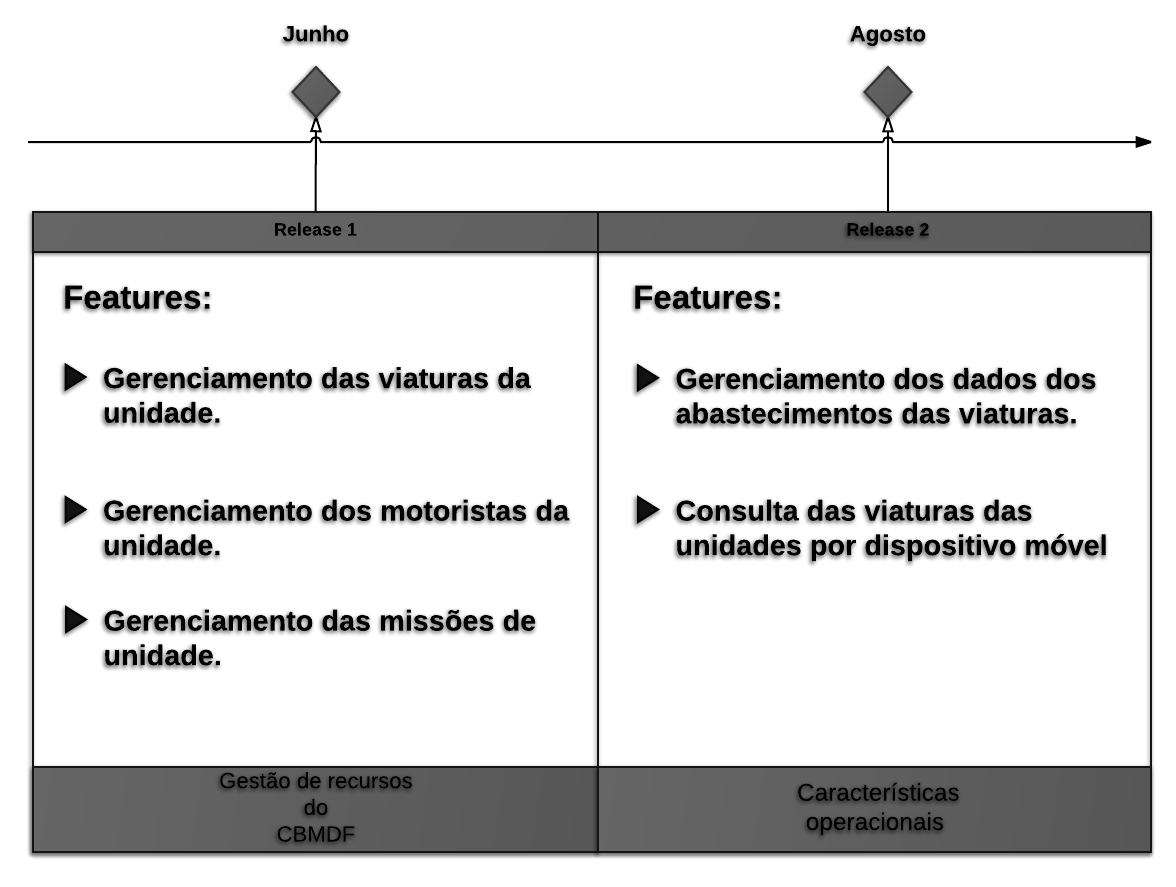
\includegraphics[scale=0.4, angle=0]{figuras/roadmap}
    \caption[\textit{Roadmap} do projeto.]{\textit{Roadmap} do projeto.}
    \label{fig:roadmap}
  \end{figure}
  
  Como ilustrado da Figura \ref{fig:roadmap}, o \textit{Roadmap} do projeto é composto por duas \textit{releases} com seus
  respectivos temas e datas. As \textit{features} foram alocadas e priorizadas, nas \textit{releases} a partir dos critérios: 
  
  \begin{itemize}
   \item Dependência funcional entre os requisitos;
    \subitem As \textit{features} estão alocadas em ordem de dependência funcional (de cima para baixo), bem como entre as
    \textit{releases} (da esquerda para direita).
    
   \item Importância relativa das mesmas para o cliente.
    \subitem As \textit{features} alocadas na \textit{release} 1 possuem maior importância e agregam maior valor ao cliente.
  \end{itemize}

    
    \subsection{Visão}
    
      O conteúdo primário da Visão de um sistema é o conjunto de features priorizadas que descrevem o que o sistema será capaz de oferecer 
      a seus usuários, para atender as necessidades dos envolvidos. \cite{leffingwell11}
      
      A visão do sistema acordada entre os \textit{stakeholders} encontra-se no documento de visão no apêndice \ref{doc_visao}
      
      \vfill